\chapter{Cơ sở lý thuyết} \label{chap-Concept}

% \input{chapters/concept_linear_algebra}
% \section{Các khái niệm về tài chính}
\subsection{Tính thanh khoản (Liquidity)}
% https://www.binance.vision/economics/liquidity-explained

% Liquidity as a term is defined as the ability to buy or sell assets in the market without causing a drastic change in the assets price.
Khái niệm về tính thanh khoản dùng để chỉ mức độ mà một tài sản có thể được mua hoặc bán trên thị trường mà không làm ảnh hưởng nhiều đến giá thị trường.
% Liquidity can refer to two different areas; liquid market and liquid asset.
% Liquid market means that there are always investors in the market willing to trade. A liquid asset refers to an asset that can be easily converted into cash.
Khái niệm tính thanh khoản được chia thành 2 loại: tính thanh khoản thị trường (liquid market) và tính thanh khoản về tài sản (liquid asset). Thị trường có tính thanh khoản cao ám chỉ rằng trong thị trường thường xuyên có các nhà đầu tư sẵn sàng giao dịch. Một tài sản có tính thanh khoản cao đồng nghĩa với việc tài sản đó có thể chuyển đổi sang tiền mặt một cách dễ dàng. Đối với thị trường tiền mã hóa, để so sánh tính thanh khoản giữa các sàn trong cùng một thời điểm hoặc tính thanh khoản của một sàn tại những thời điểm khác nhau có 3 yếu tố quan trọng: 
%24 hour trading volume, Order book depth and the amount by which the ask price exceeds the bid price, also known as the bid/ask spread.
\begin{itemize}
	\item Lượng đồng giao dịch trong ngày.
	\item Số lượng lệnh mua/bán dựa trên danh sách lệnh (order book) được công khai dựa theo các sàn như Coinbase Pro\cite{live-order-book}, Binance, Bittrex, \dots
	\item Lượng chênh lệch giữa giá yêu cầu của bên bán và giá bỏ thầu của bên mua (bid/ask spread).
\end{itemize}

\subsection{Nhiễu (Noise)}
Khái niệm nhiễu có quan hệ đối lập với khái niệm thông tin (information) với dữ liệu giá cung cấp đầy đủ thông tin, việc dự đoán dễ dàng và ngược lại với dữ liệu có nhiễu cao do bị ảnh hưởng bởi các yếu tố khác như phần đề cập tại phần \ref{overview:factor}. Nhiễu khiến những quan sát của các nhà đầu tư không được hoàn hảo, điều này dẫn thị trường có khả lưu động\cite{noise-finance}.


% \section{Các khái niệm về xác suất}
\subsection{Hàm mật độ xác suất (Probability density function)}
Với các phiên giao dịch có các thành phần như giá mở, giá đóng, số lượng đồng giao dịch,\dots, ta có thể coi như các biến ngẫu nhiên liên tục tương ứng. Khái niệm hàm mật độ xác suất trong văn cảnh trên được hiểu như một hàm gồm các tham số thể hiện được mật độ phân bố của các biến ngẫu nhiên.
\begin{figure}[hbt!]
	\center	\includegraphics[width=0.8\textwidth]{probability/z_score_marginal_distribute_diff.png}
	\caption{Phân phối biên giá mở/đóng dữ liệu đã xử lý}
	\label{fig:z_score_marginal_distribution_diff}
\end{figure}
\FloatBarrier
Hình ~\ref{fig:z_score_marginal_distribution_diff} thể hiện mật độ của phân phối đồng thời giữa giá đóng và giá mở của các khối nến được biểu diễn dưới dạng $p_{data}(Open, Close)$.
\subsection{Hàm phân phối biên (Marginal distribution)}
Với dữ liệu liên tục như trên, hàm phân phối biên đối với giá mở được biểu diễn dưới dạng:
$p_{data}(Open) = \int_y p_{data}(Open, Close=y) dy = \int_y p_{data}(Open \given Close=y)p_{data}(Close=y)dy$ Một cách trực quan, hàm phân phối trên được biểu diễn bởi đường biên bên trái Hình ~\ref{fig:z_score_marginal_distribution_diff}

\subsection{Nhiễu trắng (White noise)}
Nhiễu trong dữ liệu như phần đề cập trong phần \ref{concept:finance:noise} có thể được giảm thiểu bằng cách tìm hàm phân phối của nhiễu bằng thống kê, nếu phân phối của nhiễu có dạng phân phối chuẩn với trung bình là 0, nhiễu này được gọi là nhiễu trắng Gauss (white Gaussian noise). Việc giảm thiểu nhiễu trong dữ liệu làm mô hình trở nên dễ tìm được mẫu đặc trưng (pattern) hơn.

\subsection{Biến ẩn (Latent variable)}
Biến ẩn được hiểu theo cách trừu tượng là biến không thể quan sát trực tiếp\cite[trang~264]{bishop} mà được suy luận từ biến quan sát được trong dữ liệu. Cụ thể hơn, với dữ liệu là giá của 100 ngày đầu một mô hình có khả năng tìm được quan hệ giữa giá ngày thứ 50 phụ thuộc nhiều vào giá ngày thứ 49 hơn so với ngày thứ 99, mô hình này được gọi là mô hình biến ẩn (latent variable model) với quan hệ được biểu diễn bằng phép toán có giá trị được lưu trong các biến ẩn.
\subsection{Mô hình đồ thị có hướng (Directed graphical model)}
Trong mô hình đồ thị có hướng hay mạng Bayes (Bayes network) việc suy diễn từ các trạng thái trước sang các trạng thái sau.
\begin{figure}[hbt!]
	\center	\includegraphics[width=0.6\textwidth]{Variational_inference/Bayes_inference.png}
	\caption{Mô hình mạng Bayes}
	\label{fig:Bayes_inference}
\end{figure}
Cụ thể với mô hình được được trực quan theo như Hình ~\ref{fig:Bayes_inference}, một giao dịch BTC/USD vào 6 giờ sáng ngày 31/7/2017 có giá mở là 2439.97\$, giá đóng là 2415.19\$, lượng giao dịch là 138.82 đồng BTC với xu hướng giao dịch tiếp theo có xác suất được kí hiệu là:
$P(Up \given Open =2727.26, Close=2740.01, Volume BTC = 385.41)$ với xác suất đồng thời của giao dịch và được tính:
%\begin{equation} \label{eq1}
%\begin{multline*}
\begin{equation}
\begin{split}
p(Up,Open = 2727.26, Close = 2740.01, Volume BTC = 385.41)\\
= p(Open = 2727.26) \cdot p(Close = 2740.01) \cdot p(Volume BTC = 385.41)\\
\cdot p(Pa(Up) \given Open =2727.26, Close=2740.01, Volume BTC = 385.41)\\
\cdot p(P_1 \given Open =2727.26, Close=2740.01, Volume BTC = 385.41)\\
\cdot p(Up \given Pa(Up), P_1)
\end{split}
\end{equation}



Một cách tổng quát xác suất đồng thời của giao dịch và xu hướng tăng giảm về giá của giao dịch tiếp theo được biểu diễn dưới dạng:
$p_\theta(x_1, x_2, \dots, x_M) = \prod_{i=1}^{M}p_\theta(x_j, Pa(x_j))$ với $Pa(x_j)$ giá trị của nút mạng trước đó (parent variable) của $x_j$.
\subsection{Suy luận biến phân (Variational inference)}
Phương pháp suy luận biến phân được sử dụng trong mô hình đồ thị có hướng\cite{intro_variational} với các biến ẩn $z$ và các quan sát $x$ với mục tiêu ước lượng được phân bố của $x$ được xấp xỉ bằng phân phối $Q(Z)$: $P(X \given Z) \approx Q(Z)$ với $Q(Z)$ là phân phối tiên nghiệm đơn giản hơn $P(Z|X)$.

Sử dụng độ đo bất đồng Kullback–Leibler nhằm thể hiện sự khác nhau giữa phân phối $Q$ so với phân phối $P$: 


$\Dkl{Q}{P} \triangleq  \mathbb{E}_{Q(Z)} [\log \frac{Q(Z)}{P(Z \given X)}]$

Sử dụng luật Bayes:
$\Dkl{P}{Q} = \mathbb{E}_{Q(Z)} [\log \frac{Q(z)}{P(z , x)}  + \log P(x)]$\\
hay:\\
$\log(P(x)) = \Dkl{P}{Q} - \mathbb{E}_{Q(z)} [\log \frac{Q(z)}{P(z , x)}]
= \Dkl{P}{Q} + \mathcal{L}(Q)
$


%\section{Các khái niệm về mô hình sinh, mô hình phân biệt}
Khái niệm mô hình sinh và mô hình phân biệt ở đây được sử dụng trong ngữ cảnh học có giám sát.
\subsection{Mô hình sinh (Generative Model)}
Với dữ liệu đầu vào là $x$ được gán nhãn y trong quá trình tiền xử lý, mô hình sinh học được phân bố đồng thời của x và y $p_\theta(x,y)$ thông qua việc ước lượng các giá trị của các thông số trong $\theta$ việc suy diễn nhãn đối với dữ liệu kiểm thử được thực hiện bằng cách sử dụng luật Bayes\cite{gen-vs-dis} để tính $p_\theta(y\given x)$ sau đó tính giá trị dự đoán của nhãn với $\hat{y}$ có độ tin cậy cao nhất:
$\hat{y} = \argmax\limits_{y \in \mathcal{D}_y} p_\theta(y\given x)$. Với định nghĩa này một mô hình khi có đầu vào gồm các giao dịch và các thuộc tính được thêm vào từ bước xử lý dữ liệu mô hình có khả năng học được phân bố của các giao dịch và có thể sinh ra được các giao dịch mới theo phân bố tương tự như phân bố của dữ liệu được coi là mô hình sinh hay mô hình sinh mẫu.
%%%%%%%%%%%%%%%%%%%%%%%%%%%%%%%%%%%%%%%%%%%%%%%%%%%%%%%%%
\subsection{Mô hình phân biệt (Discriminative Model)}
Mô hình phân biệt học được phân bố $p_\theta(y \given x)$, việc suy diễn nhãn được tính trực tiếp từ dữ liệu kiểm thử. Với định nghĩa này một mô hình có cùng dữ liệu trên chứa thông tin của các giao dịch và đầu ra là xu hướng tăng hoặc giảm của giao dịch hoặc giá tiếp theo của giao dịch được gọi là mô hình phân biệt.
%%%%%%%%%%%%%%%%%%%%%%%%%%%%%%%%%%%%%%%%%%%%%%%%%%%%%%%%%



%\subsection{Likelihood}

% \section{Các khái niệm về xác suất}

\section{Tiền mã hóa} \label{concept:crypto-currency}
\subsection{Khái niệm về tiền mã hóa}
Tiền mã hóa là một dạng tiền tệ kỹ thuật số được tạo ra như một phương thức để trao đổi, sử dụng các phương pháp mã hóa để bảo vệ, xác minh các giao dịch cũng việc quản lý việc tạo ra các đơn vị tiền mã hóa trong hệ thống.

Tiền mã hóa sử dụng một hệ thống phân tán để quản lý thay vì một hệ thống xác thực trung tâm như các cách thức quản lý trước đây. Hệ thống phân tán này như một cuốn sổ cái phân tán, được gọi là Blockchain, đảm nhận vai trò lưu trữ các giao dịch một cách công khai đến những người tham gia. Quá trình xác minh giao dịch dựa trên sự đồng thuận phân tán. Quá trình này còn gọi là đào (mining).

\section{Nhiễu dữ liệu} \label{concept:noise}
Trong tài chính khái niệm nhiễu (noise) có quan hệ đối lập với khái niệm thông tin (information), với dữ liệu cung cấp đầy đủ thông tin, việc dự đoán dễ dàng và ngược lại với dữ liệu có nhiễu cao do bị ảnh hưởng bởi các yếu tố khác như đã đề cập tại Tiểu mục \ref{overview:market-noise} do các lệnh mua bán trong tương lai không tuân theo các quy luật từ giao dịch trước đó. Việc khử nhiễu dữ liệu là loại bỏ các yếu tố trên, nhằm cho việc tìm luật chung được dễ dàng hơn. %tìm một luật chung cho dữ liệu (pattern) sao cho trên tập kiểm thử vẫn tuân theo pattern của các phiên giao dịch trước.

\section{Hàm mật độ xác suất}
Với các phiên giao dịch có các thành phần như giá mở, giá đóng, số lượng đồng giao dịch,\dots ta có thể coi như các biến ngẫu nhiên liên tục tương ứng. Khái niệm hàm mật độ xác suất (probability density function) trong văn cảnh trên được hiểu như một hàm gồm các tham số thể hiện được mật độ phân bố của các biến ngẫu nhiên.
\begin{figure}[hbt!]
	\center	\includegraphics[width=0.6\textwidth]{figures/probability/z_score_marginal_distribute_diff.png}
	\caption{Phân phối biên giá mở/đóng dữ liệu đã xử lý}
	\label{fig:z_score_marginal_distribution_diff}
\end{figure}
\FloatBarrier
Hình ~\ref{fig:z_score_marginal_distribution_diff} thể hiện mật độ của phân phối đồng thời giữa giá đóng và giá mở của các khối nến được biểu diễn dưới dạng $p_{data}(Open, Close)$.
\section{Hàm phân phối biên}
Với dữ liệu liên tục như trên, hàm phân phối biên (marginal distribution) đối với giá mở được biểu diễn dưới dạng:

%\begin{align}
\begin{gather}
\label{mat}
p_{data}(Open) = \int_y p_{data}(Open, Close=y) dy = \int_y p_{data}(Open \given Close=y)p_{data}(Close=y)dy 
\end{gather}

 
 
 

%\end{align}

Một cách trực quan, hàm phân phối trên được biểu diễn bởi đường biên bên trái Hình ~\ref{fig:z_score_marginal_distribution_diff}

\section{Nhiễu trắng}
Khái niệm nhiễu có thể được giảm thiểu bằng cách tìm hàm phân phối của nhiễu bằng thống kê, nếu phân phối của nhiễu có dạng phân phối chuẩn với trung bình là 0, nhiễu này được gọi là nhiễu trắng Gauss (white Gaussian noise). Việc giảm thiểu nhiễu trong dữ liệu làm mô hình trở nên dễ tìm được mẫu đặc trưng (pattern) hơn.

\section{Biến ẩn}
Biến ẩn (Latent variable) được hiểu theo cách trừu tượng là biến không thể quan sát trực tiếp\cite[trang~264]{bishop} 
mà được suy luận từ biến quan sát được trong dữ liệu. Cụ thể hơn, với dữ liệu là giá của 10 ngày đầu một mô hình có khả năng tìm được quan hệ giữa giá ngày thứ 5 phụ thuộc nhiều vào giá ngày thứ 4 hơn so với ngày thứ 9, mô hình này được gọi là mô hình biến ẩn (latent variable model) với quan hệ được biểu diễn bằng phép toán có giá trị được lưu trong các biến ẩn.
\section{Mô hình đồ thị có hướng}
Trong mô hình đồ thị có hướng (directed graphical model) hay mạng Bayes (Bayes network) việc suy diễn từ các trạng thái trước sang các trạng thái sau.
\begin{figure}[hbt!]
	\center	\includegraphics[width=0.6\textwidth]{figures/Variational_inference/Bayes_inference.png}
	\caption{Mô hình mạng Bayes}
	\label{fig:Bayes_inference}
\end{figure}
Cụ thể với mô hình được được trực quan theo như Hình ~\ref{fig:Bayes_inference}, một giao dịch BTC/USD vào 6 giờ sáng 2017/7/31/ có giá mở là 2439.97\$, giá đóng là 2415.19\$, lượng giao dịch là 138.82 đồng BTC với xu hướng giao dịch tiếp theo có xác suất được kí hiệu là:
\begin{align*}
 P(Up \given Open =2727.26, Close=2740.01, Volume BTC = 385.41)   
\end{align*} với xác suất đồng thời của giao dịch và được tính:
%\begin{equation} \label{eq1}
\begin{align*}
p(Up,Open = 2727.26, Close = 2740.01, Volume BTC = 385.41)\\
= p(Open = 2727.26) \cdot p(Close = 2740.01) \cdot p(Volume BTC = 385.41)\\
\cdot p(Pa(Up) \given Open =2727.26, Close=2740.01, Volume BTC = 385.41)\\
\cdot p(P_1 \given Open =2727.26, Close=2740.01, Volume BTC = 385.41)\\
\cdot p(Up \given Pa(Up), P_1)
% \end{split}
% \end{equation}
\end{align*}

Một cách tổng quát xác suất đồng thời của giao dịch và xu hướng tăng giảm về giá của giao dịch tiếp theo được biểu diễn dưới dạng:
\begin{align*}
p_\theta(x_1, x_2, \dots, x_M) = \prod_{i=1}^{M}p_\theta(x_j, Pa(x_j))
\end{align*}

với $Pa(x_j)$ giá trị của nút mạng trước đó (parent variable) của $x_j$.
\subsection{Phương pháp cận dưới biến phân}\label{variational-lower-bound}
% Phương pháp suy luận biến phân  (Variational inference) được sử dụng trong mô hình đồ thị có hướng\cite{intro_variational} với các biến ẩn $z$ và các quan sát $x$ với mục tiêu ước lượng được phân bố của $x$ được xấp xỉ bằng phân phối $Q(Z)$: $P(X \given Z) \approx Q(Z)$ với $Q(Z)$ là phân phối tiên nghiệm đơn giản hơn $P(Z|X)$.
Để giải quyết hàm bất trị (intractable function) trong Tiểu mục \ref{eq:intractable_likelihood}, ta có thể dùng phương pháp cận dưới biến phân \cite[trang~198]{intro_variational} (Variational lower bound). Chi tiết phương pháp đi từ việc xấp xỉ likelihood:

% Phương pháp suy luận biến phân được sử dụng để xấp xỉ 
\begin{align}
    \log p_\theta(x^{(i)})
    &= \mathbb{E}_{z} \left[\log p_\theta(x^{(i)} \right] \label{eq:11}\\
    &= \mathbb{E}_{z} \left[\log \frac{p_\theta(x^{(i)} \given z)p_\theta(z)}
    {p_\theta(z \given x^{(i)})} \right] \label{eq:12}\\
    &= \mathbb{E}_{z} \left[\log \frac{p_\theta(x^{(i)} \given z)p_\theta(z)}
    {p_\theta(z \given x^{(i)})}  
    \frac{q_\phi(z\given x^{(i)})} {q_\phi(z\given x^{(i)})} 
    \right]\\
    &=\mathbb{E}_{z} \left[\log p_\theta(x^{(i)} \given z) \right]
    - \mathbb{E}_{z} \left[\log \frac{q_\phi(z \given x^{(i)})}{p_\theta(z)} \right]
    + \mathbb{E}_{z} \left[\log \frac{q_\phi(z \given x^{(i)})}{p_\phi(z \given x^{(i)})} \right]\\
    &= \mathcal{L}(x^{(i)}, \theta, \phi) 
    + \Dkl{q_\phi(z \given x^{(i)})}{p_\phi(z \given x^{(i)})} 
\end{align}

%phuong trinh 11 \eqref{eq:11}
%phuong trinh 12 \eqref{eq:12}
Với $\Dkl{q_\phi(z \given x^{(i)})}{p_\phi(z \given x^{(i)})}$
còn được gọi là độ đo bất đồng Kullback–Leibler nhằm thể hiện sự khác nhau giữa hai phân phối $q_\phi(z \given x^{(i)})$ và $p_\phi(z \given x^{(i)})$.
Một cách tổng quát độ đo bất đồng Kullback–Leibler giữa phân phối $Q$ so với phân phối $P$ mang giá trị không âm và được tính như sau: 
\begin{align}
\Dkl{Q}{P} \triangleq  \mathbb{E}_{Q(Z)} \left[\log \frac{Q(Z)}{P(Z \given X)}\right] \geq 0
\end{align}
Sử dụng luật Bayes:
\begin{align}
\Dkl{P}{Q} = \mathbb{E}_{Q(Z)} \left[\log \frac{Q(z)}{P(z , x)}  + \log P(x)\right]
\end{align}
hay:
\begin{align}
\log(P(x)) = \Dkl{P}{Q} - \mathbb{E}_{Q(z)} \left[\log \frac{Q(z)}{P(z , x)}\right]
= \Dkl{P}{Q} + \mathcal{L}(Q)
\end{align}
